\chapter{Metodologia}
\label{chap:mat}

Um dos pontos característico do programa de Formação em Robótica é a sua metodologia, onde buscará a aprendizagem ativa do estudante, com a construção dos seus conhecimentos, complementando as aulas expositivas com atividades e dinâmicas de grupo, elaboração e apresentação de trabalhos e pesquisas, emprego de meios audiovisuais, estudos individualizados, pesquisa de artigos técnicos e científicos, entre outros condicionantes ao programa.
A metodologia em si é um caminho para o sucesso na formação dos estudantes, pois esta convergência baseia-se em 5 pontos principais:

\begin{enumerate}
    \item \textbf{Criatividade:} espaço que estimula a criatividade, possibilitando interação e acesso à diferentes tecnologias.
    \item \textbf{Engajamento:} atividades práticas de aprendizado aumentam os níveis de concentração
    \item \textbf{Programação:} a inteligência artificial se torna cada vez mais presente nas escolas e escritórios
    \item \textbf{Trabalho em equipe:} robótica incorpora uma gama de habilidades e promove um ambiente de aprendizagem para pessoas com diferentes talentos
    \item \textbf{Diversão:} aprender sobre robótica deve ser divertido, e a medida que os estudantes continuem melhorando sua interação com eles, isso aumenta mais ainda o nível de diversão
\end{enumerate}


Basicamente o caminho para o sucesso compreende em 4 fases distintas, demonstradas na Figura \ref{fig:metodologia}:

\textbf{Assimilação:} desenvolver habilidades de codificação e lógica;

\textbf{Simulação:} testar as missões de um robô de forma eficiente;

\textbf{Integração:} garantir informações sobre o ambiente e o robô;

\textbf{Criação:} elaborar um projeto aplicado a tecnologia.

As três primeiras fases são compreendidas em 6 meses, ficando a fase Criação com 6 meses para finalizar o programa.
Entre cada fase, desafios são lançados para que o estudante obtenha maior sucesso na assimilação dos conceitos ministrados, para a última fase um projeto final é lançado para que o estudante possa realizar a demonstração de seu sistema para os avaliadores.
Bom salientar que durante as fases, temas serão tratados e discutidos de forma expositiva e prática.


\begin{figure}[H]
    \caption{Metodologia do Programa de Formação em Robótica e Sistemas Autônomos}
    \centering
    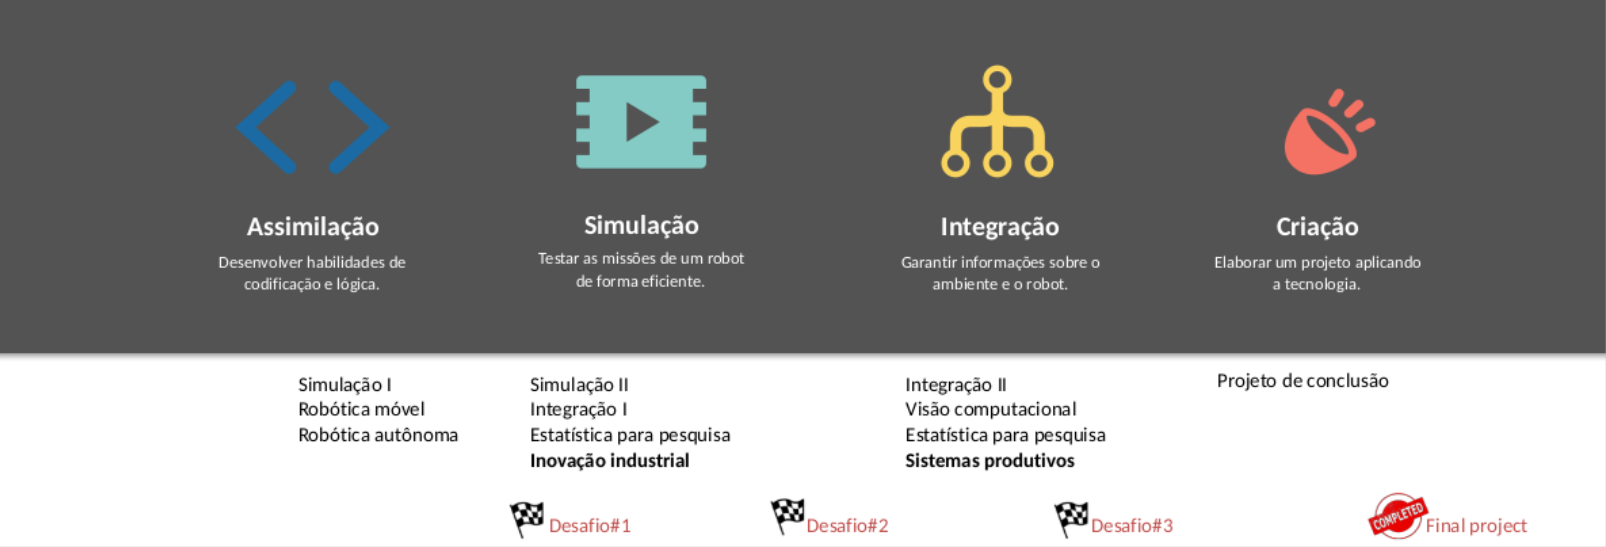
\includegraphics[width= \textwidth]{Figures/metodologia.png}
    \caption*{Fonte: Programa de Formação em Robótica e Sistemas Autônomos}
    \label{fig:metodologia}
\end{figure}

Com uma abordagem inovadora, o programa tenta realçar a busca por um aprendizado mais real e excitante para isso o conceito de professor facilitador que estimule a experiência nas várias tecnologias se faz necessário. Isso promoverá vários feedbacks mais intensos aos estudantes. Em resumo o professor será o facilitador de uma experiência de aprendizado, criando recursos e experiência para a formação do aprendiz.